\documentclass[aspectratio=169,11pt]{beamer}

% ---- Minimalist theme (same style family as midway slides) ----
\usetheme{default}
\usecolortheme{default}
\setbeamertemplate{navigation symbols}{}
\setbeamertemplate{frametitle continuation}{}
\setbeamertemplate{itemize items}[circle]
\setbeamertemplate{enumerate items}[default]

% ---- Font: TeX Gyre Heros ----
\usepackage[T1]{fontenc}
\usepackage{tgheros}
\renewcommand{\familydefault}{\sfdefault}
\usepackage{microtype}

% ---- Packages ----
\usepackage{amsmath}
\usepackage{booktabs}
\usepackage{array}
\usepackage{tikz}
\usepackage{xcolor}
\usepackage{hyperref}
\usepackage{listings}
\usetikzlibrary{arrows.meta,positioning,calc,fit,decorations.pathreplacing}

% ---- Maastricht University colors ----
\definecolor{umdark}{HTML}{001C3D}
\definecolor{umorange}{HTML}{E84E10}
\definecolor{umlight}{HTML}{4A90C4}
\definecolor{umgray}{HTML}{6B7280}
\definecolor{umbg}{HTML}{F8F9FA}
\definecolor{umfaint}{HTML}{E5E7EB}
\definecolor{umgreen}{HTML}{16A34A}
\definecolor{umcoral}{HTML}{DC4A3C}

% ---- Apply colors to Beamer ----
\setbeamercolor{normal text}{fg=umdark}
\setbeamercolor{frametitle}{fg=umdark}
\setbeamercolor{title}{fg=umdark}
\setbeamercolor{subtitle}{fg=umgray}
\setbeamercolor{author}{fg=umgray}
\setbeamercolor{date}{fg=umgray}
\setbeamercolor{institute}{fg=umorange}
\setbeamercolor{itemize item}{fg=umorange}
\setbeamercolor{itemize subitem}{fg=umlight}
\setbeamercolor{enumerate item}{fg=umorange}
\setbeamercolor{block title}{bg=umdark,fg=white}
\setbeamercolor{block body}{bg=umdark!5,fg=umdark}
\setbeamercolor{block title alerted}{bg=umorange,fg=white}
\setbeamercolor{block body alerted}{bg=umorange!8,fg=umdark}
\setbeamercolor{block title example}{bg=umlight,fg=white}
\setbeamercolor{block body example}{bg=umlight!8,fg=umdark}

% ---- Listing style ----
\lstset{
  basicstyle=\ttfamily\scriptsize,
  keywordstyle=\color{umdark},
  commentstyle=\color{umgray},
  stringstyle=\color{umorange},
  backgroundcolor=\color{umbg},
  frame=single,
  rulecolor=\color{umfaint},
  breaklines=true,
  showstringspaces=false,
  columns=fullflexible
}

% ---- Frametitle style ----
\setbeamertemplate{frametitle}{%
  \vspace{0.35cm}%
  \noindent\hspace*{0pt}%
  \parbox{\textwidth}{%
    {\usebeamerfont{frametitle}\usebeamercolor[fg]{frametitle}\insertframetitle}%
    \vspace{2pt}\\%
    {\color{umorange}\rule{\textwidth}{1.2pt}}%
  }%
  \vspace{-2pt}%
}
\setbeamerfont{frametitle}{size=\large,series=\bfseries}
\setbeamersize{text margin left=0.7cm,text margin right=0.7cm}

% ---- Footline (page number only) ----
\setbeamertemplate{footline}{%
  \hbox{%
    \begin{beamercolorbox}[wd=\paperwidth,ht=2.2ex,dp=1ex]{footline}%
      \hfill%
      {\scriptsize\color{umgray}\insertframenumber/\inserttotalframenumber}%
      \hspace{1em}%
    \end{beamercolorbox}%
  }%
}

% ---- Metadata ----
\title{Carrier Origin and\\Steganographic Detectability}
\subtitle{Does the source of an image change how easily we can detect hidden data?}
\newcommand{\teamauthors}{Abdul Moiz Akbar \;|\; Malo Coquin \;|\; Daria Gjonbalaj \;|\; Nico Muller-Spath\\Jimena Narvaez del Cid \;|\; David Wicker \;|\; Nikolas Zouros}
\author[Project 2.2 Team]{Project 2.2 Team}
\institute{Department of Advanced Computing Sciences\\Maastricht University}
\date{Project 2.2 \;|\; March 2026}

\begin{document}

% ============================================================
% SLIDE 1 — Title
% ============================================================
\begin{frame}[plain]
\vfill
\begin{center}
{\color{umorange}\rule{0.42\textwidth}{2pt}}\\[12pt]
{\LARGE\bfseries\color{umdark}\inserttitle}\\[10pt]
{\normalsize\color{umgray}\insertsubtitle}\\[16pt]
{\small\color{umdark}\teamauthors}\\[8pt]
{\small\color{umorange}\insertinstitute}\\[8pt]
{\footnotesize\color{umgray}\insertdate}\\[12pt]
{\color{umorange}\rule{0.42\textwidth}{2pt}}
\end{center}
\vfill
\end{frame}

% ============================================================
% SLIDE 2 — The Big Picture
% ============================================================
\begin{frame}{The Big Picture}
\begin{columns}[T]
\begin{column}{0.52\textwidth}
\begin{block}{The intuition}
Hiding data in an image shifts its statistical fingerprint --- even by a tiny amount, detectors can pick it up.
\end{block}
\vspace{0.2cm}
\begin{alertblock}{The twist}
What if that fingerprint was \textbf{already different} before any data was embedded? AI-generated images and real photographs may not look the same to a detector, even in their unmodified state.
\end{alertblock}
\end{column}
\begin{column}{0.44\textwidth}
\centering
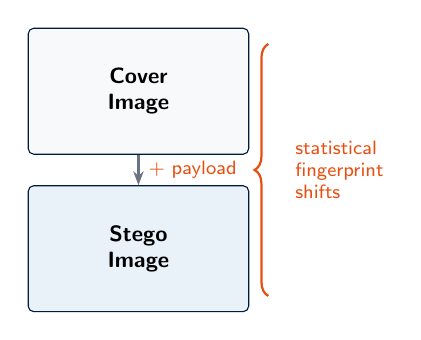
\begin{tikzpicture}[
    box/.style={draw=umdark, fill=umbg, rounded corners=2pt,
                minimum width=2.8cm, minimum height=1.6cm,
                font=\footnotesize\bfseries, align=center},
    arr/.style={-{Stealth[length=5pt]}, thick, color=umgray},
    lbl/.style={font=\tiny, color=umgray}
]
  % Cover image
  \node[box] (cover) at (0,2) {Cover\\Image};
  % Embedding arrow
  \node[lbl, right=0.15cm of cover] (emb) {};
  % Stego image
  \node[box, fill=umlight!12] (stego) at (0,0) {Stego\\Image};
  % Arrow
  \draw[arr] (cover) -- node[right, font=\scriptsize, color=umorange] {+ payload} (stego);
  % Fingerprint shift
  \draw[decorate, decoration={brace, amplitude=5pt, mirror},
        thick, color=umorange]
    (1.65,2.6) -- (1.65,-0.6)
    node[midway, right=6pt, font=\scriptsize, color=umorange, align=left]
    {statistical\\fingerprint\\shifts};
\end{tikzpicture}
\end{column}
\end{columns}

\vspace{0.15cm}
\begin{center}
\fcolorbox{umorange}{umorange!6}{%
  \parbox{0.88\textwidth}{\centering\scriptsize\color{umdark}%
    \textbf{Core question:} Does the \emph{origin} of the carrier --- real photo vs.\ AI-generated --- change how easily we detect hidden data?%
  }%
}
\end{center}
\end{frame}

% ============================================================
% SLIDE 3 — Research Questions
% ============================================================
\begin{frame}{Research Questions}
\small
\renewcommand{\arraystretch}{1.35}
\begin{tabular}{@{}c >{\raggedright}p{2.6cm} c p{7.2cm}@{}}
\toprule
 & \textbf{Question} & \textbf{Type} & \textbf{Description} \\
\midrule
\textcolor{umorange}{\textbf{RQ1}} & Carrier Source &
  \tikz\node[fill=umlight!15, rounded corners=2pt, inner sep=2pt, font=\tiny\bfseries, text=umlight]{Primary}; &
  Does carrier source (real vs.\ ML-generated) affect detectability under matched embedding? \\
\textcolor{umorange}{\textbf{RQ2}} & Generator Effect &
  \tikz\node[fill=umlight!15, rounded corners=2pt, inner sep=2pt, font=\tiny\bfseries, text=umlight]{Primary}; &
  Within ML carriers, does the choice of generator (SDXL vs.\ FLUX.1) matter? \\
\textcolor{umorange}{\textbf{RQ3}} & Payload Interaction &
  \tikz\node[fill=umorange!12, rounded corners=2pt, inner sep=2pt, font=\tiny\bfseries, text=umorange]{Exploratory}; &
  Does increasing payload size widen or close the detectability gap? \\
\textcolor{umorange}{\textbf{RQ4}} & Embedding Branch &
  \tikz\node[fill=umorange!12, rounded corners=2pt, inner sep=2pt, font=\tiny\bfseries, text=umorange]{Exploratory}; &
  Do spatial (LSB + PNG) and frequency (DCT + JPEG) branches show different effects? \\
\textcolor{umorange}{\textbf{RQ5}} & Encryption Invariance &
  \tikz\node[fill=umgreen!15, rounded corners=2pt, inner sep=2pt, font=\tiny\bfseries, text=umgreen]{Verification}; &
  Does AES-256-CBC encryption of the payload affect detectability? \\
\bottomrule
\end{tabular}

\vspace{0.35cm}
\begin{center}
\small\color{umgray} These five questions structure the entire experiment and map directly to pipeline outputs.
\end{center}
\end{frame}

% ============================================================
% SLIDE 4 — Prototype Design
% ============================================================
\begin{frame}{Prototype}
\begin{columns}[T]
\begin{column}{0.47\textwidth}
\begin{block}{Vertical Prototype --- Depth}
Each core component implemented and tested in isolation:
\begin{itemize}
  \item \textbf{LSB embedding} --- configurable fill rate and bit depth
  \item \textbf{AES-256-CBC encryption} --- payload-level crypto
  \item \textbf{3 statistical detectors:}\\
    Chi-Square, RS Analysis, Sample Pairs
\end{itemize}
\end{block}
\vspace{0.1cm}
{\scriptsize\color{umgray} Proves each component works independently.}
\end{column}
\begin{column}{0.47\textwidth}
\begin{block}{Horizontal Prototype --- Breadth}
All components wired into one pipeline running across \textbf{60 images}:
\end{block}
\vspace{0.1cm}
\centering
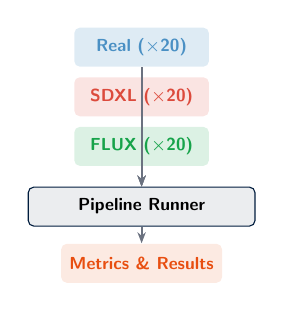
\begin{tikzpicture}[scale=0.9, every node/.style={scale=0.9},
    src/.style={draw=none, rounded corners=2pt, minimum width=1.9cm,
                minimum height=0.55cm, font=\scriptsize\bfseries, align=center},
    pipe/.style={draw=umdark, fill=umdark!8, rounded corners=2pt,
                 minimum width=3.2cm, minimum height=0.55cm,
                 font=\scriptsize\bfseries},
    arr/.style={-{Stealth[length=4pt]}, thick, color=umgray}
]
  \node[src, fill=umlight!18, text=umlight] (real) at (0,1.6) {Real ($\times$20)};
  \node[src, fill=umcoral!15, text=umcoral] (sdxl) at (0,0.9) {SDXL ($\times$20)};
  \node[src, fill=umgreen!15, text=umgreen] (flux) at (0,0.2) {FLUX ($\times$20)};
  \node[pipe] (pipe) at (0,-0.65) {Pipeline Runner};
  \draw[arr] (real.south) -- ++(0,-0.1) -| (pipe.north);
  \draw[arr] (sdxl.south) -- (pipe.north);
  \draw[arr] (flux.south) -- ++(0,-0.1) -| (pipe.north);
  \node[src, fill=umorange!12, text=umorange] (met) at (0,-1.45) {Metrics \& Results};
  \draw[arr] (pipe.south) -- (met.north);
\end{tikzpicture}

\vspace{0.05cm}
{\tiny\color{umgray} Proves all parts work together; early results across all five RQs.}
\end{column}
\end{columns}
\end{frame}

% ============================================================
% SLIDE 5 — Code Architecture
% ============================================================
\begin{frame}{Code Architecture}
\begin{columns}[T]
\begin{column}{0.50\textwidth}
\small
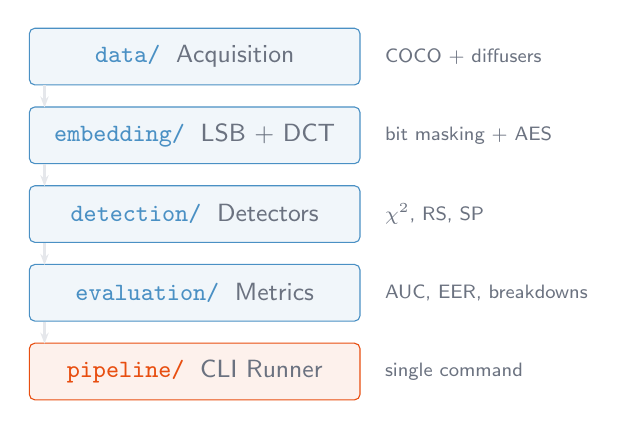
\begin{tikzpicture}[
    pkg/.style={draw=umlight, fill=umlight!8, rounded corners=2pt,
                minimum width=4.2cm, minimum height=0.72cm,
                font=\small, align=left, anchor=west},
    desc/.style={font=\scriptsize, color=umgray, anchor=west},
    arr/.style={-{Stealth[length=4pt]}, thick, color=umfaint}
]
  % Packages stacked
  \node[pkg] (acq) at (0,4) {\texttt{\textbf{\textcolor{umlight}{data/}}} \;\textcolor{umgray}{Acquisition}};
  \node[desc] at (4.4,4) {COCO + diffusers};

  \node[pkg] (emb) at (0,3) {\texttt{\textbf{\textcolor{umlight}{embedding/}}} \;\textcolor{umgray}{LSB + DCT}};
  \node[desc] at (4.4,3) {bit masking + AES};

  \node[pkg] (det) at (0,2) {\texttt{\textbf{\textcolor{umlight}{detection/}}} \;\textcolor{umgray}{Detectors}};
  \node[desc] at (4.4,2) {$\chi^2$, RS, SP};

  \node[pkg] (eva) at (0,1) {\texttt{\textbf{\textcolor{umlight}{evaluation/}}} \;\textcolor{umgray}{Metrics}};
  \node[desc] at (4.4,1) {AUC, EER, breakdowns};

  \node[pkg, draw=umorange, fill=umorange!8] (pip) at (0,0)
    {\texttt{\textbf{\textcolor{umorange}{pipeline/}}} \;\textcolor{umgray}{CLI Runner}};
  \node[desc] at (4.4,0) {single command};

  % Connecting arrows
  \draw[arr] (acq.south west) ++(0.2,0) -- ++(0,-0.28);
  \draw[arr] (emb.south west) ++(0.2,0) -- ++(0,-0.28);
  \draw[arr] (det.south west) ++(0.2,0) -- ++(0,-0.28);
  \draw[arr] (eva.south west) ++(0.2,0) -- ++(0,-0.28);
\end{tikzpicture}
\end{column}
\begin{column}{0.46\textwidth}
\begin{exampleblock}{Launching the viewer}
\vspace{0.05cm}
{\ttfamily\scriptsize
\textcolor{umgreen}{\$} pip install -r requirements.txt\\
\textcolor{umgreen}{\$} python viewer.py\\
\textcolor{umgray}{Serving Stego Explorer on \textcolor{umlight}{http://localhost:8765}}\\
\textcolor{umgray}{Press Ctrl+C to stop.}%
}
\vspace{0.05cm}
\end{exampleblock}

\vspace{0.15cm}
\begin{block}{What the viewer provides}
\scriptsize
\begin{itemize}
  \item Runs overview with source-effect delta
  \item Per-run detail: config, results, gallery, conditions
  \item RQ-organized analysis cards with AUC bars
  \item Per-image detector scores and cover/stego comparison
  \item Context-aware search across all pages
\end{itemize}
\end{block}
\end{column}
\end{columns}
\end{frame}

\end{document}
